%%%%%%%%%%%%%%%%%%%%%%%%%%%%%%%%%%%%%%%%%%%%%%%%%%%%%%%%%%%%%%%%%%%%%%%%%%%%% 
%
% This is a LaTeX file for an A0 poster.
% 
% template poster taken from https://canizo.org/latex_poster
%
%%%%%%%%%%%%%%%%%%%%%%%%%%%%%%%%%%%%%%%%%%%%%%%%%%%%%%%%%%%%%%%%%%%%%%%%%%%%% 

%%%%%%%%%%%%%%%%%%%%%%%%%%%%%%%%%%%%%%%%%%%%%%%%%%%%%%%%%%%%%%%%%%%%%%%%%%%%% 
%%%%%%%%%%%%%%%%%%%%%%%%%%%%%%%%%%%%%%%%%%%%%%%%%%%%%%%%%%%%%%%%%%%%%%%%%%%%%
%
% scpdata: a data package for single-cell proteomics
%
% Poster for the Eurobioc2019, December 2019.
%
%%%%%%%%%%%%%%%%%%%%%%%%%%%%%%%%%%%%%%%%%%%%%%%%%%%%%%%%%%%%%%%%%%%%%%%%%%%%%
%%%%%%%%%%%%%%%%%%%%%%%%%%%%%%%%%%%%%%%%%%%%%%%%%%%%%%%%%%%%%%%%%%%%%%%%%%%%%

\documentclass{article}
% To modify the size of the page:
\usepackage[dvips,a3paper,portrait,centering,margin=0.4cm]{geometry}
% To create multiple columns
\usepackage{multicol}

\usepackage[utf8]{inputenc}
% To align images
\usepackage[export]{adjustbox}
% Use captions in minipages
\usepackage{caption}
% Math font
\usepackage{amsmath, amsthm, amsfonts}
% Include figure files.
\usepackage{graphicx}

% Coding fonts
% ------------
% For including R chunks 
\usepackage{listings} 
\lstset{
  language=R,
  basicstyle=\small\ttfamily\color{vdgray},       % the size of the fonts that are used for the code
  % sensitive=false,
  numbers=left,                   % where to put the line-numbers
  numberstyle=\tiny\color{gray},  % the style that is used for the line-numbers
  stepnumber=1,                   % the step between two line-numbers.
  numbersep=0.1cm,                % how far the line-numbers are from the code
  backgroundcolor=\color{lgray},  % choose the background color. You must add \usepackage{color}
  deletekeywords={stat},
  keywordstyle=\color{blue},      % keyword style
  stringstyle=\color{green},      % string literal style
  xleftmargin=0.5cm,
}
% Create command for highlighting inline code or variables
\newcommand{\hcode}[2][lgray]{{\ttfamily\color{vdgray}\colorbox{#1}{#2}}}

% Colors
% ------
\usepackage{color}
\usepackage[dvipsnames]{xcolor}
% Color panel used throughout the poster
\definecolor{lgray}{rgb}{0.9179688,0.9179688,0.9179688} % #ebebeb
\definecolor{dgray}{rgb}{0.796875,0.796875,0.796875} % #cccccc
\definecolor{vdgray}{rgb}{0.3984375,0.3984375,0.3984375} % #666666
\definecolor{coral}{rgb}{0.9960938,0.4960938,0.3125000} % #ff7f50
\definecolor{blue}{rgb}{0.4218750,0.6484375,0.8007812} % #6ca6cd
\definecolor{green}{rgb}{0.6992188,0.7265625,0.5078125} % #b3ba82
\definecolor{yellow}{rgb}{0.9570312,0.8671875,0.6992188} % #f5deb3

% Adjust space between reference items
% ------------------------------------
\let\OLDthebibliography\thebibliography
\renewcommand\thebibliography[1]{
  \OLDthebibliography{#1}
  \setlength{\parskip}{0pt}
  \setlength{\itemsep}{0pt plus 0.3ex}
}
  
\pagestyle{empty}

\def\to{\rightarrow}


% ===========================================================================

\title{}
\author{}
\date{}

\begin{document}


% ---------------------------------------------------------------------------
% Banner


\begin{center}
\colorbox{lgray}{
  \begin{minipage}{3cm}
    \includegraphics[width=1.2\linewidth]{figs/DSC_2812.jpg}
  \end{minipage}
  %&
  \begin{minipage}{.74\textwidth}
    \begin{center}
      % Title 
      \huge \textbf{scpdata: a data package for single-cell proteomics} \\
      \vspace{0.4cm}
      % Authors
      \Large \textbf{Christophe Vanderaa, Laurent Gatto} \\
      % Affiliation
      \Large \textit{Computational biology and bioinformatics lab, de Duve Institute, UCLouvain } \\
      % email
      \vspace{0.4cm}
      \normalsize christophe.vanderaa@uclouvain.be \\
    \end{center}
  \end{minipage}
  %&
  \begin{minipage}{3.7cm}
      
\includegraphics[width=0.7\linewidth, right]{figs/fnrs.png} \\
      \vspace{0.5cm}
      
\includegraphics[width=1.1\linewidth, right]{figs/ucl.png}
  \end{minipage}
}
\end{center}


% ------------------------\---------------------------------------------------
% Summary

\setlength{\columnsep}{1cm}
\begin{multicols}{2}

\noindent
\fcolorbox{yellow}{yellow}{
  \begin{minipage}[t]{\linewidth}
      \vspace{.15cm}
      \section*{\huge Summary}
      \large Recent advances in sample preparation, processing and mass spectrometry (MS) have allowed the emergence of MS-based single-cell proteomics (SCP). However, bioinformatics tools to process and analyze these new types of data are still missing. In order to boost the development and the benchmarking of SCP methodologies, we are developing the \hcode[yellow]{scpdata} experiment package. The package will distribute published and curated SCP data sets in standardized Bioconductor format. 
    
  \end{minipage}
}
\noindent

% ---------------------------------------------------------------------------
% Introduction
\noindent
\begin{minipage}[t]{\linewidth}
  \vspace{0.55cm}
  \section*{\huge Introduction}
  \large
  
  There are two main pipelines able to generate MS-SCP data:

  \begin{itemize}
    \item \textbf{\large nanoPOTS pipeline} (Zhu et al., 2018, \cite{Zhu2018-bf}) runs label-free proteomics for single cells. The \textbf{\color{BrickRed}{throughput is low}} ($\pm$ 10 samples/day), but achieves \textbf{\color{OliveGreen}{accurate peptide quantification}}. 
    \vspace{-0.5cm}
    \begin{center}
      
\includegraphics[width=0.87\linewidth]{figs/nanopots.png} \\
    \end{center}
    \vspace{-0.5cm}
    \item \textbf{\large SCoPE pipeline} (Slavov Lab, 2018, \cite{Budnik2018-qh}) adapts TMT-based proteomics to single-cells. The \textbf{\color{OliveGreen}{throughput is higher}} ($\pm$ 5 samples/hour), but \textbf{\color{BrickRed}{presence of chemical noise}}.
    \vspace{-0.5cm}
    \begin{center}
      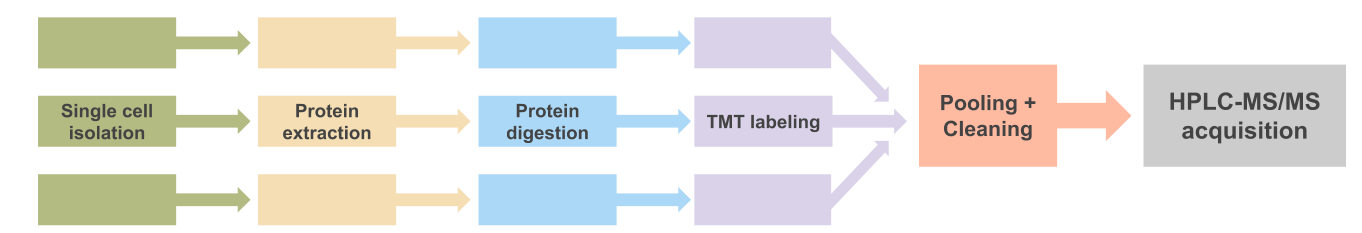
\includegraphics[width=0.9\linewidth]{figs/scopems.png} \\
    \end{center}
  \end{itemize}
  
\end{minipage}

% ---------------------------------------------------------------------------
% Content of the package
\noindent
\begin{minipage}[t]{\linewidth}
  \vspace{0.55cm}
  \section*{\huge Content of the package}
  
  \large
  \hcode{scpdata} contains SCP data sets formatted as \hcode{MSnbase::MSnSet} objects. The package provides data at \textbf{peptide} and \textbf{protein} level. \textbf{Help files} are provided for every data set and accessed using \hcode{?dou2019\_1\_protein}. Available data sets are listed using \hcode{scpdata()}.
  
  \scriptsize
  \begin{tabular}{@{\extracolsep{5pt}} cl} 
    \\[-1.8ex]\hline 
    \hline \\[-1.8ex] 
    \textbf{Item} & \textbf{Title} \\ 
    \hline \\[-1.8ex] 
    dou2019\_1\_protein & FACS + nanoPOTS + TMT multiplexing: HeLa digests (Dou et al. 2019) \\ 
    dou2019\_2\_protein & FACS + nanoPOTS + TMT multiplexing: testing boosting ratios (Dou et al. 2019) \\ 
    dou2019\_3\_protein & FACS + nanoPOTS + TMT multiplexing: profiling of murine cell populations (Dou... \\
    specht2018\_peptide & SCoPE-MS + mPOP lysis upgrade: Master Mix 20180824 (Specht et al. 2018) \\ 
    specht2019\_peptide & FACS + SCoPE2: comparing macrophages against monocytes (Specht et al. 2019) \\ 
    specht2019\_peptide2 & FACS + SCoPE2: comparing macrophages against monocytes (Specht et al. 2019) \\ 
    specht2019\_protein & FACS + SCoPE2: comparing macrophages against monocytes (Specht et al. 2019) \\ 
    \hline \\[-1.8ex] 
  \end{tabular} 
  
\end{minipage}
  

% ---------------------------------------------------------------------------
% Data manipulation
\noindent
\begin{minipage}[t]{\linewidth}
  \vspace{0.55cm}
  \section*{\huge Data manipulation}
  \large
  
  The Bioconductor class \hcode{MSnSet} is a reliable framework for standard and systematic data processing. Below, the re-implementation of the R script provided in \cite{Specht2019-jm}:
  

  \begin{lstlisting}
    data("specht2019_peptide")
    specht2019_peptide %>% 
      scp_normalize_stat(what = "row", mean, "-") %>%
      scp_aggregateByProtein() %>%
      scp_normalize_stat(what = "column", median, "-") %>%
      scp_normalize_stat(what = "row", mean, "-") %>%
      imputeKNN(k = 3) %>%
      batchCorrect(batch = "raw.file", target = "celltype") -> scpd
  \end{lstlisting}
  
\end{minipage}

  

% ---------------------------------------------------------------------------
% Data quality control
\noindent
\begin{minipage}[t]{\linewidth}
  \vspace{0.55cm}
  \section*{\huge Data quality control}
  \large
  When developing the SCoPE technology, the Slavov lab also suggested some quality control (QC) measures and visualizations \cite{Huffman2019-ns} (eg Figure \ref{fig:qc}). The \hcode{scpdata} package provides an ideal data environment for developing and improving SCP data QC.
  \begin{center}
    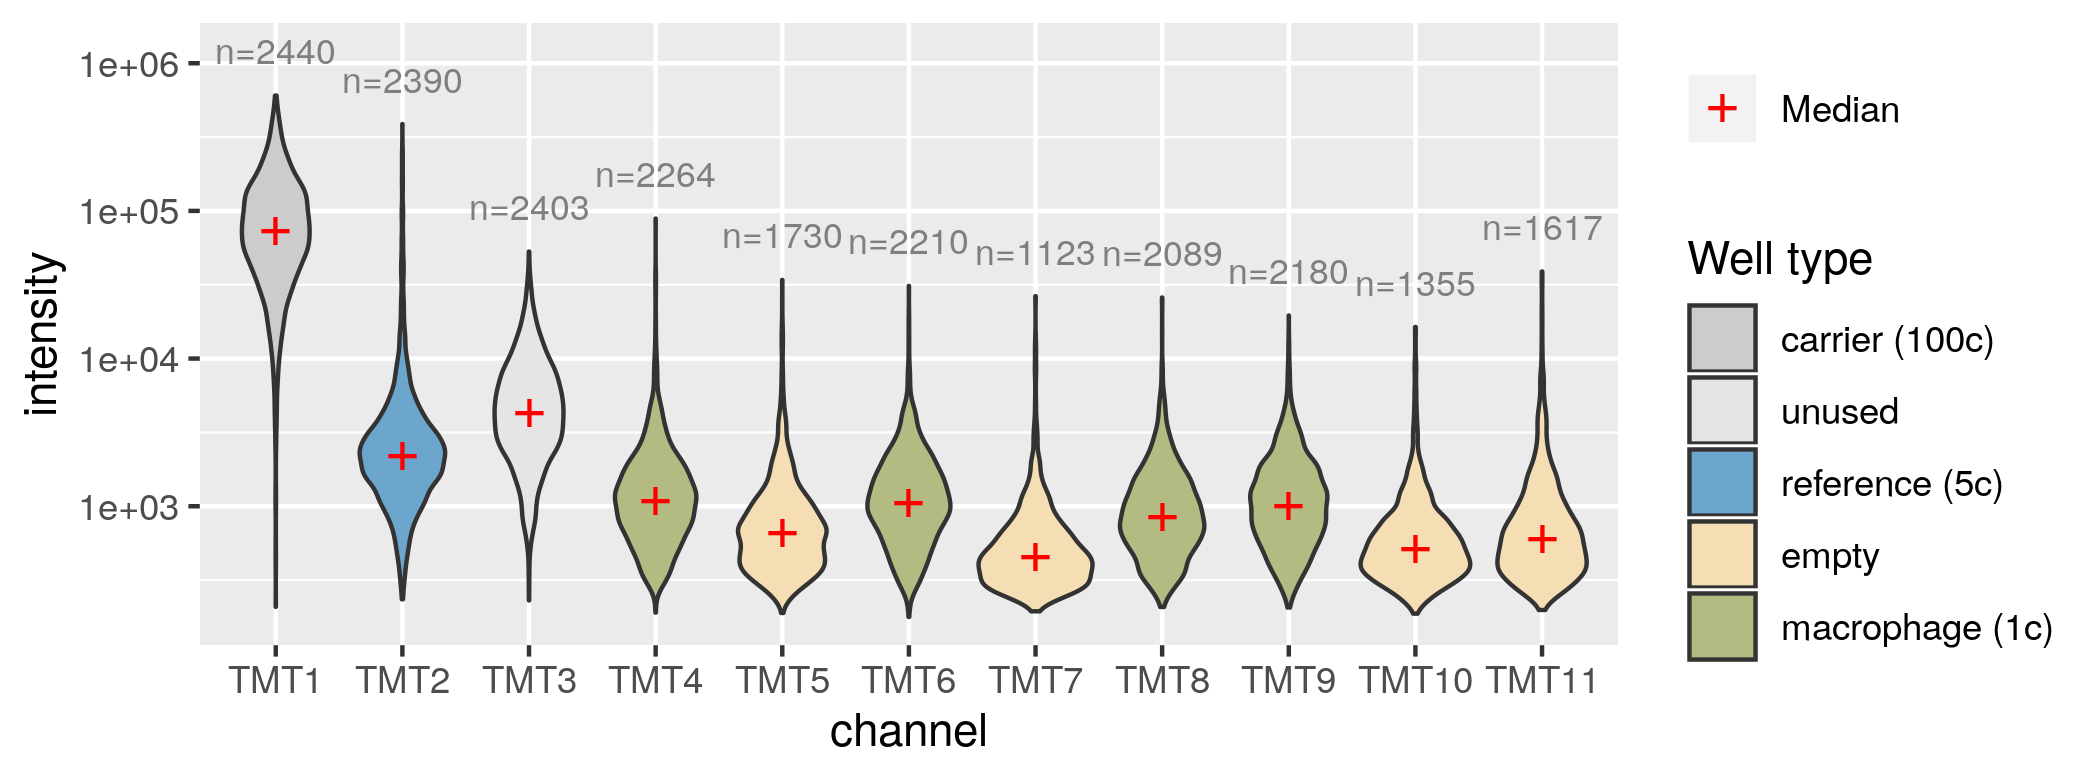
\includegraphics[width=0.95\textwidth]{figs/QC.png}
  \end{center}
  \vspace{-0.5cm}
  \captionof{figure}{\textbf{MS intensity distributions per channel at peptide level.} \small Contamination peptides or peptides with a low identification score were removed. Data taken from run \hcode{190222S\_LCA9\_X\_FP94BF} published in \cite{Specht2019-jm}. n: number of non-missing peptides.}
  \label{fig:qc}
\end{minipage}



% ---------------------------------------------------------------------------
% Benchmarking
\noindent
\begin{minipage}[t]{\linewidth}
  \vspace{0.4cm}
  \section*{\huge Benchmarking}
  \large
  \hcode{scpdata} also offers an ideal environment for benchmarking. It will contain a wide variety of MS-SCP data sets from \textbf{well-defined synthetic standards} to \textbf{real biological samples}. When phenotype information is available, \textbf{objective benchmarking metrics} can be used for comparing different methods. \textbf{Visualization with dimension reduction} (PCA, tSNE, UMAP) are also part of the benchmarking process (Figure \ref{fig:pca}).
  \begin{center}
    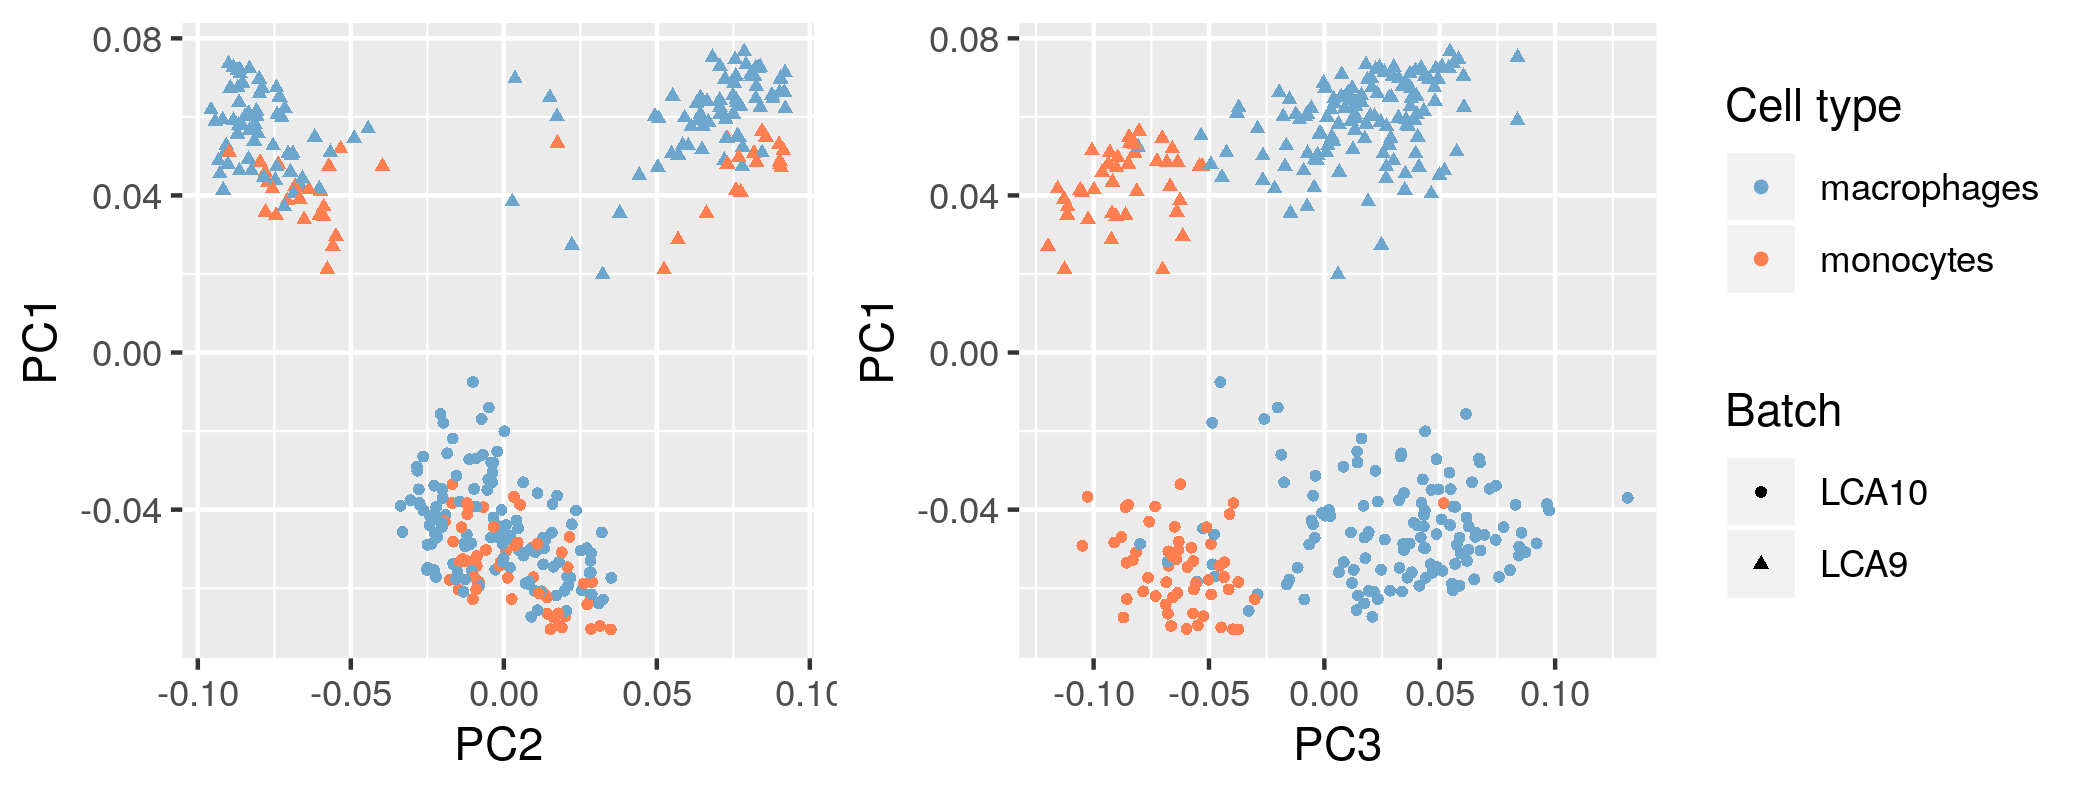
\includegraphics[width=\textwidth]{figs/PCA.png}
  \end{center}
  \captionof{figure}{\textbf{PCA plot of peptide expression data.} \small Macrophages and monocytes are well separated in the third principal component. However, the first and second components are driven by batch effects. LCA10 and LCA9 are two chromatographic batches. The PCA was performed using the NIPALS algorithm.}
  \label{fig:pca}

\end{minipage}

% ---------------------------------------------------------------------------
% Problems to tackle: batch effect
\noindent
\begin{minipage}[t]{\linewidth}
  \vspace{0.55cm}
  \section*{\huge Problems to tackle}
  \subsection*{Batch effects}
  \large
  Batch effects are inherent to MS-SCP data since many samples/cells have to be distributed across \textbf{different MS runs} (even with TMT labeling). This leads to tremendous batch effects (Figure \ref{fig:pca}).
  
\end{minipage}
  
% ---------------------------------------------------------------------------
% Problems to tackle: Missingness
\noindent
\vspace{0.4cm}
\begin{minipage}[h]{0.37\linewidth}
  \subsection*{Missingness}
  \large
  The data sets in \cite{Specht2019-jm} contains $\pm$ 75 \% missing data. Missingness can impact downstream analyses and must be handled thoroughly as different sample types can exhibit different proportion of missing data (Figure \ref{fig:missing}).
\end{minipage}
\hspace{0.4cm}
\begin{minipage}[h]{0.6\linewidth}
  \begin{center}
    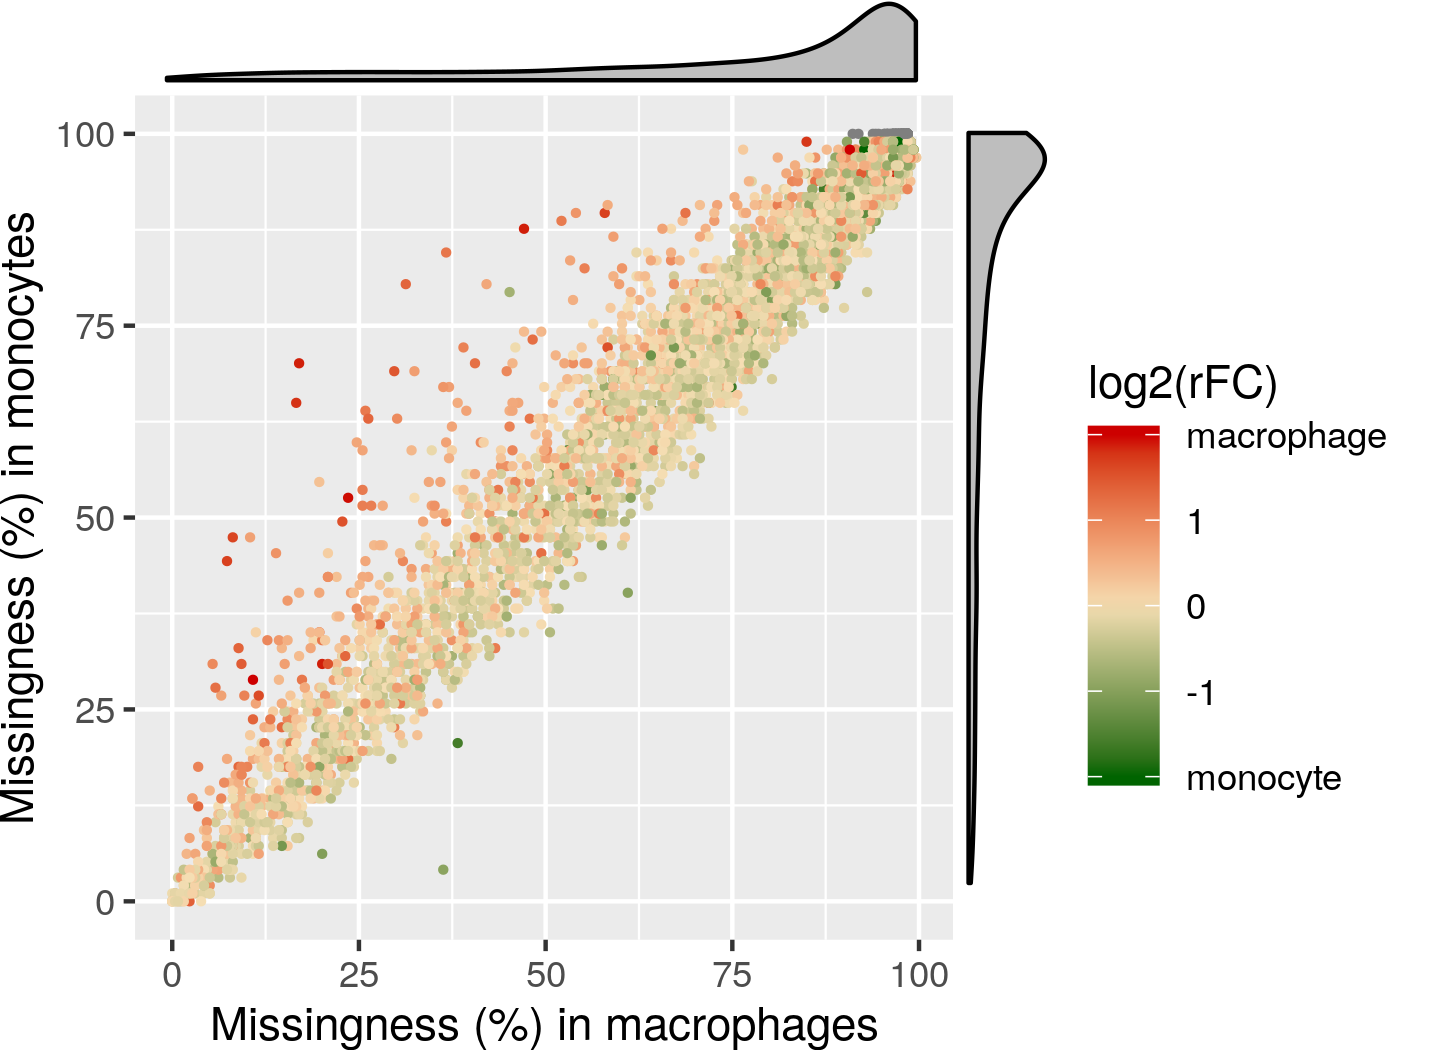
\includegraphics[width=\linewidth]{figs/missing.png}
  \end{center}
\end{minipage}
\noindent
\begin{minipage}[h]{\linewidth}
  \captionof{figure}{\textbf{Distribution of missing data in monocytes against macrophages.} \small Color indicates the log2 fold change of \textbf{\color{coral}macrophages} over \textbf{\color{green}monocytes} relative expression.}
  \label{fig:missing}
\end{minipage}

% ---------------------------------------------------------------------------
% Problems to tackle: Curse of dimensionality
\noindent
\begin{minipage}[t]{\linewidth}
  \subsection*{Curse of dimensionality}
  \large
  Although current acquisition pipelines produce data sets of \textbf{thousands of peptides x hundreds of cells}, it is expected that new technological advances might raise the dimensionality 100 fold \cite{Specht2019-jm}. This is a challenge for the \textbf{statistical analyses} and for the \textbf{software optimization}. Possible solutions should be inspired from current achievements in single cell transcriptomics. 
\end{minipage}

% ---------------------------------------------------------------------------
% Conclusion
\vspace{.4cm}
\noindent
\colorbox{yellow}{
  \begin{minipage}[t]{0.965\linewidth}
    \vspace{.15cm}
    \section*{\huge Conclusion}
    \large 
    MS-based SCP is still at its infancy. However, we hope that developing an MS-SCP data package will provide a strong framework for bioinformatics research. It will support the development of new packages for tackling the statistical issues (missing data, batch effect, high dimensionality) seen in MS-SCP data, as well as providing a growing data repository for software benchmarking. By thorough implementation and benchmarking of its software, MS-SCP could become a new state-of-the-art technique for single-cell omcis.
  \end{minipage}
}

% ---------------------------------------------------------------------------
% References
\scriptsize
\bibliography{ref.bib} 
\bibliographystyle{ieeetr}


\end{multicols}

\end{document}